\documentclass[runningheads]{llncs}

\usepackage[T1]{fontenc}
\usepackage{graphicx}
\usepackage{amsmath,amssymb,amsfonts}
\usepackage{booktabs}
\usepackage{multirow}
\usepackage{array}
\usepackage{tabularx}
\usepackage{url}
\urlstyle{rm}

\begin{document}

\title{Concept--Latent Space Alignment in Fuzzy Attention Networks for Safety-Critical Intelligent Decision Support}

\titlerunning{Concept--Latent Space Alignment in FAN-Based IDSS}

\author{
A. N. Averkin\inst{1} \and
Yu. V. Trofimov\inst{2,3} \and
M. D. Lebedev\inst{5} \and
A. S. Ilin\inst{4} \and
E. S. Kondrashova\inst{3} \and
A. D. Lebedev\inst{3}
}

\authorrunning{A. N. Averkin et al.}

\institute{
Federal Research Center ``Computer Science and Control'' of the Russian Academy of Sciences, Moscow, Russian Federation \and
Joint Institute for Nuclear Research, Dubna, Russian Federation \and
Dubna State University, Dubna, Russian Federation \and
Innopolis University, Innopolis, Russian Federation \and
National University of Science and Technology MISIS, Moscow, Russian Federation
}

\maketitle

\begin{abstract}
Safety-critical intelligent decision support requires not only predictive accuracy but also transparent decision formation. Classical expert and fuzzy systems provide interpretable reasoning, yet scale poorly in data-rich environments, whereas deep models learn effectively from complex signals but usually remain weakly connected to semantically meaningful concepts. This study proposes a concept-oriented framework that integrates latent representation learning, a concept-consistent intermediate layer, and Fuzzy Attention Network (FAN)-based concept aggregation. In the proposed formulation, decisions are formed not directly from hidden features but through weighted concept-level evidence, making the resulting output analyzable through concept activations and their contribution to the final prediction. A prototype implementation was evaluated in two safety-relevant scenarios: anomaly-aware monitoring and degradation-aware risk prediction. The results indicate that the proposed organization maintains competitive predictive performance while providing an internally interpretable mechanism of decision formation. These findings support the feasibility of concept-oriented, FAN-based intelligent decision support as a basis for safety-critical applications.

\keywords{Explainable artificial intelligence \and intelligent decision support systems \and fuzzy attention networks \and concept space alignment \and latent space alignment \and safety-critical systems}
\end{abstract}

\section{Introduction}

Safety-critical intelligent decision support systems are expected to provide not only accurate predictions, but also decision mechanisms that can be inspected, justified, and related to domain-level reasoning. In industrial monitoring, energy infrastructure, nuclear-related applications, cyber-physical systems, and equipment health assessment, an intelligent model cannot be treated merely as a statistical predictor. Its recommendations may influence operational decisions under uncertainty, and therefore the model must support traceability of how a decision has been formed \cite{schwalbe2024criticalxai}. In such settings, the opacity of a predictive model is not only a limitation of usability, but also a factor that restricts its admissibility as a component of expert-supported decision making.

This requirement exposes a persistent methodological tension. Classical expert systems and fuzzy decision support systems are naturally interpretable because they operate with explicit concepts, linguistic variables, rule structures, and transparent aggregation schemes. However, their reliance on manually specified knowledge makes them difficult to scale to high-dimensional, noisy, and dynamically changing environments \cite{onwujekwe2025idss}. Deep neural models address this limitation from the opposite direction. They learn latent representations directly from data and can capture nonlinear temporal and structural dependencies that are difficult to encode by hand. This has made deep learning effective in anomaly detection, condition monitoring, forecasting, and degradation-aware classification. Attention-based architectures, and transformer models in particular, have further strengthened the ability of neural models to represent complex dependencies through adaptive weighting mechanisms \cite{vaswani2017attention}. Nevertheless, the internal latent spaces of such models usually remain weakly connected to concepts that domain experts can interpret and validate \cite{schwalbe2024criticalxai}.

The problem is therefore not reducible to a simple opposition between interpretable and non-interpretable models. A more fundamental issue is the absence of a stable and operational relation between learned latent representations and a semantically meaningful concept space. In safety-critical decision support, the model should not only produce a correct output, but should also indicate which interpretable system states contributed to that output and how strongly they influenced the final decision. Concept-based approaches, including concept bottleneck models, demonstrate the importance of introducing intermediate semantic variables between the input and the final prediction \cite{koh2020cbm}. However, a concept bottleneck alone does not fully determine how concept-level evidence should be weighted, aggregated, and transformed into a decision under uncertainty. In particular, dynamic safety-relevant environments require not only concept prediction, but also context-dependent assessment of concept relevance.

A related line of work investigates the integration of fuzzy logic and attention mechanisms in neural architectures. Fuzzy attention is attractive for safety-critical decision support because it can represent graded relevance rather than purely discrete rule activation or opaque feature weighting. Recent studies suggest that fuzzy attention mechanisms can improve the interpretability and structural organization of neural models in transformer-like, temporal, and graph-based settings \cite{chakraborty2025fantf,zhang2025hfan,zhao2026fanl,trofimov2025fuzzytransformer}. However, existing uses of fuzzy attention often remain close to feature-level weighting. In such cases, attention may become more structured, but it is still not necessarily grounded in an explicit concept space. As a result, the model may assign weights to internal features without providing a sufficiently clear account of the semantic states that those weights represent.

The position adopted in this study is that safety-critical intelligent decision support requires an explicit organization of the relation between latent representation learning, concept-level representation, and decision formation. In the proposed formulation, the latent space is not treated as a self-sufficient substrate from which the final prediction is produced directly. Instead, latent representations are mapped into an intermediate concept space whose components correspond to semantically interpretable system states. This concept space is associated with neuro-cognitive knowledge representations, understood here as knowledge structures intended to preserve a link between learned internal representations and domain-level concepts available for expert analysis. The final decision is then formed through Fuzzy Attention Network (FAN)-based aggregation of concept-level evidence rather than through direct classification of hidden features.

The key distinction of the proposed approach is that FAN is not used as a generic attention module over latent features. It is reformulated as a mechanism for weighting and aggregating concept activations. In this setting, concepts represent interpretable states of the monitored system, while FAN weights represent the context-dependent contribution of these states to the final decision. Thus, the explanation is not introduced as a post hoc approximation of a black-box model. Instead, it follows from the internal decision structure: the model output can be analyzed through the activated concepts and their weighted contributions. This organization separates the proposed framework both from standard concept bottleneck models, where concept variables may be used without a dedicated fuzzy aggregation mechanism, and from conventional attention models, where weights are usually assigned to latent features, tokens, or temporal positions rather than to semantically grounded concepts.

The study therefore proposes a concept-oriented framework that integrates latent representation learning, concept-consistent intermediate organization, and FAN-based concept aggregation into a single decision-making scheme. The contribution of the paper is threefold. First, a methodological framework is introduced in which latent representations are constrained through an intermediate concept space intended to support semantic traceability in safety-critical intelligent decision support. Second, FAN is formulated as a concept-level evidence aggregation mechanism, distinguishing it from ordinary feature-level attention and from concept bottleneck architectures without fuzzy concept weighting. Third, a prototype implementation is evaluated in two safety-relevant scenarios, anomaly-aware monitoring and degradation-aware risk prediction, in order to examine whether the proposed organization can preserve competitive predictive performance while providing an internally interpretable mechanism of decision formation.



\section{Methodology}

\subsection{Architecture of the Proposed Framework}

The proposed framework is designed to organize decision formation through an explicit transition from observations to latent representations, from latent representations to semantically grounded concepts, and from concepts to the final decision support output. The architecture consists of three main components: a trainable encoder, a concept alignment layer, and a Fuzzy Attention Network (FAN) block for concept-level evidence aggregation.

The encoder extracts a latent representation from raw multivariate observations. The concept alignment layer maps this latent representation into an intermediate concept space whose dimensions correspond to semantically interpretable system states. The FAN block then assigns context-dependent fuzzy relevance weights to these concept activations and aggregates them into a decision representation. In contrast to architectures in which the final prediction is produced directly from hidden features, the proposed model makes the concept layer a necessary stage of decision formation.

This organization is illustrated in Fig.~\ref{fig:framework_architecture}. The input observation is first processed by a trainable neural encoder, which maps the observed system state into a latent representation space. The resulting latent representation is not used directly as the final substrate of prediction. Instead, it is projected into a concept space through a concept alignment layer. The concept-level representation is then processed by a FAN block, which performs fuzzy concept weighting and aggregation. The final decision support output is produced from the aggregated concept evidence.

\begin{figure}[tbp]
    \centering
    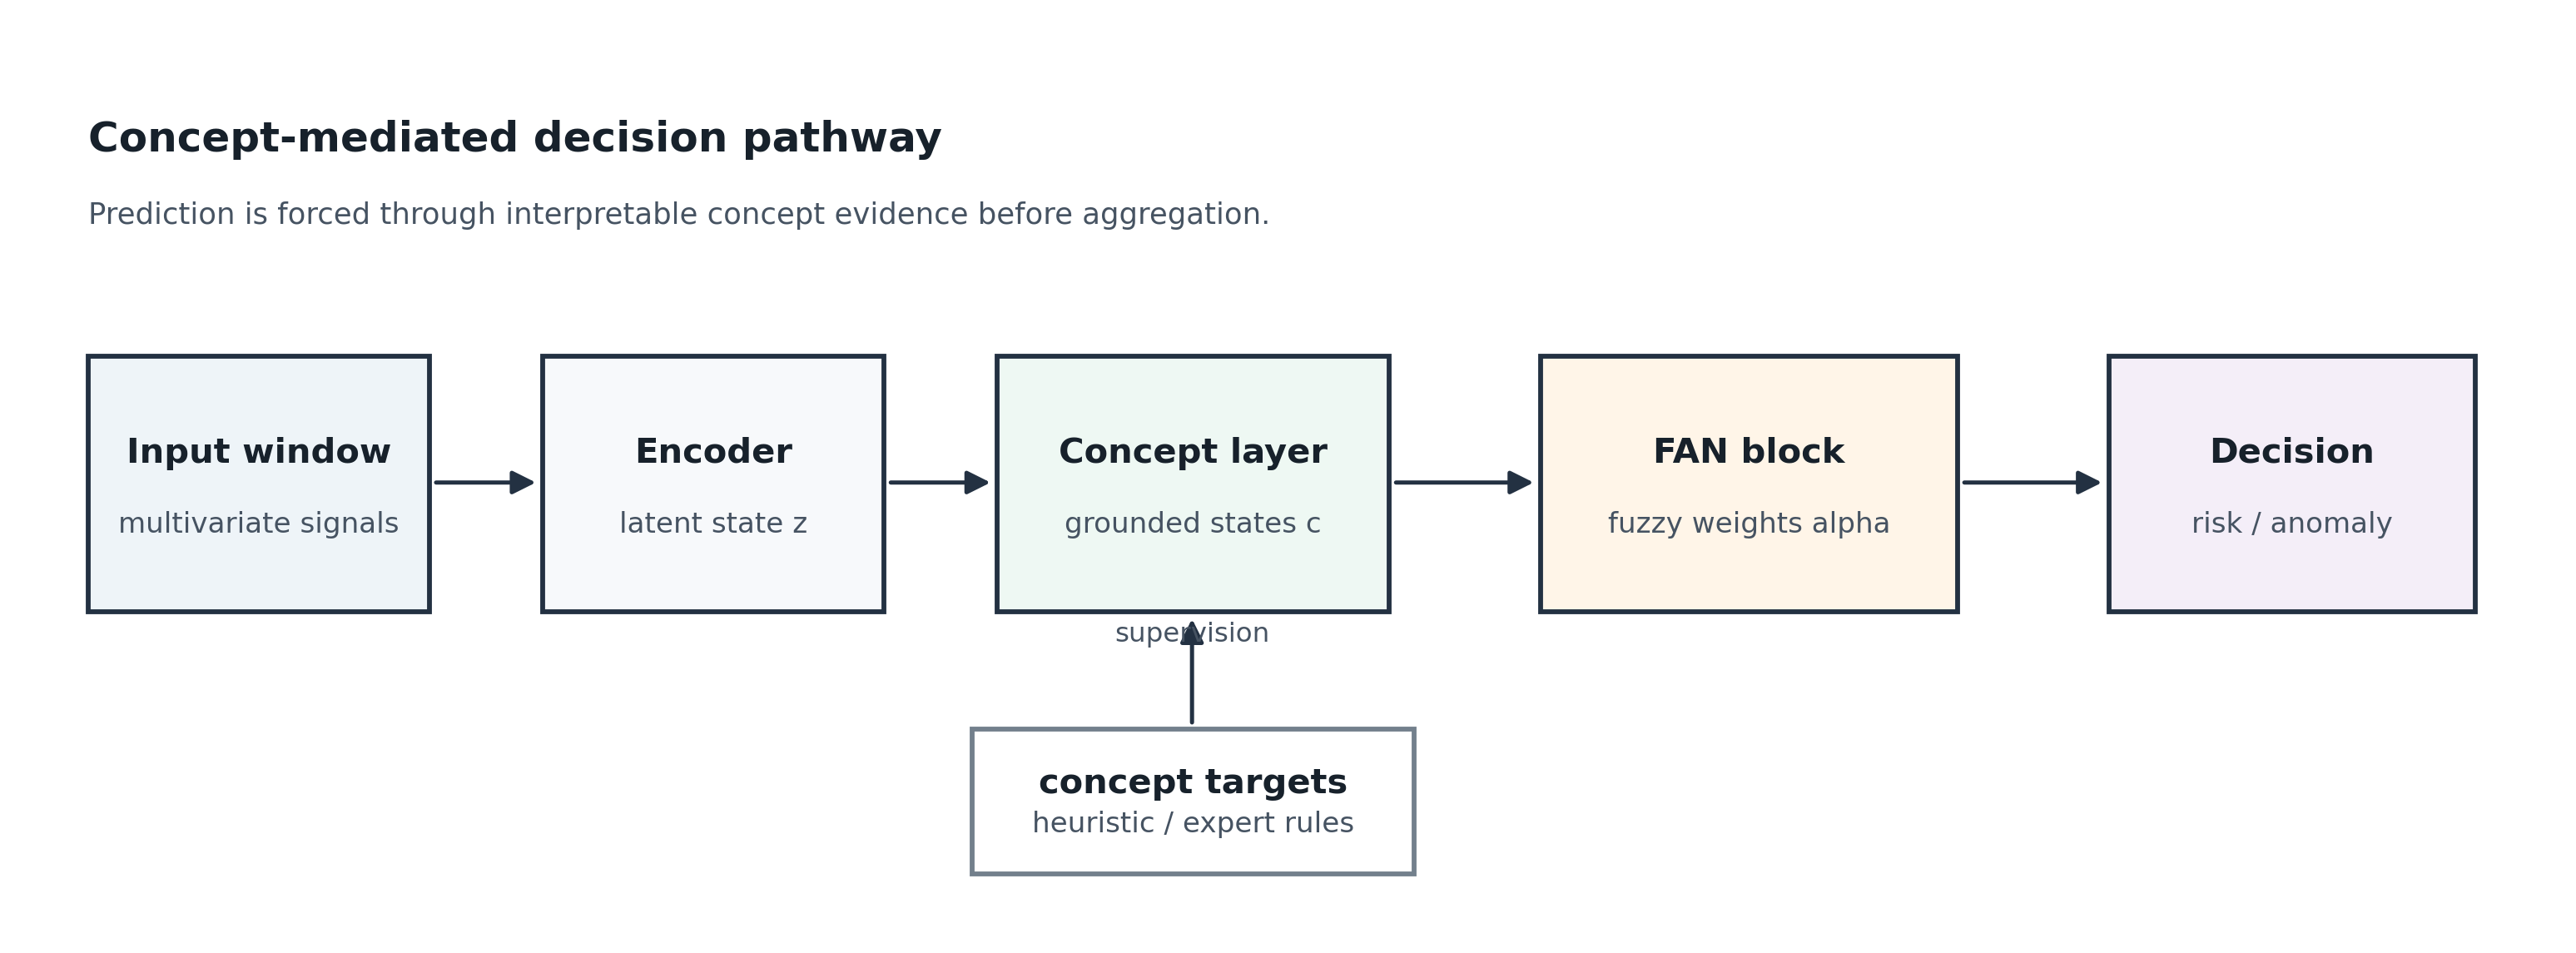
\includegraphics[width=\textwidth]{figures/framework_architecture.png}
    \caption{Concept-mediated FAN decision pathway.}
    \label{fig:framework_architecture}
\end{figure}

The central architectural distinction of the proposed system is that the decision is mediated by interpretable concept activations. The concept layer is not treated merely as a dimensionality-reduction bottleneck. It is introduced as an intermediate semantic interface between the latent representation and the decision output. Therefore, the model is required to form its decision through concept-level evidence rather than through unconstrained hidden features.

The interpretability mechanism implied by this organization is summarized in Fig.~\ref{fig:interpretability_scheme}. The explanation is derived from two complementary components: the concept-level representation, which determines \emph{what} system states are activated, and the FAN weighting structure, which determines \emph{which} of these activated states are most influential for the final decision. Consequently, interpretability is not introduced as a post hoc approximation of an already trained black-box model. It is embedded into the internal decision pathway of the architecture.

\begin{figure}[tbp]
    \centering
    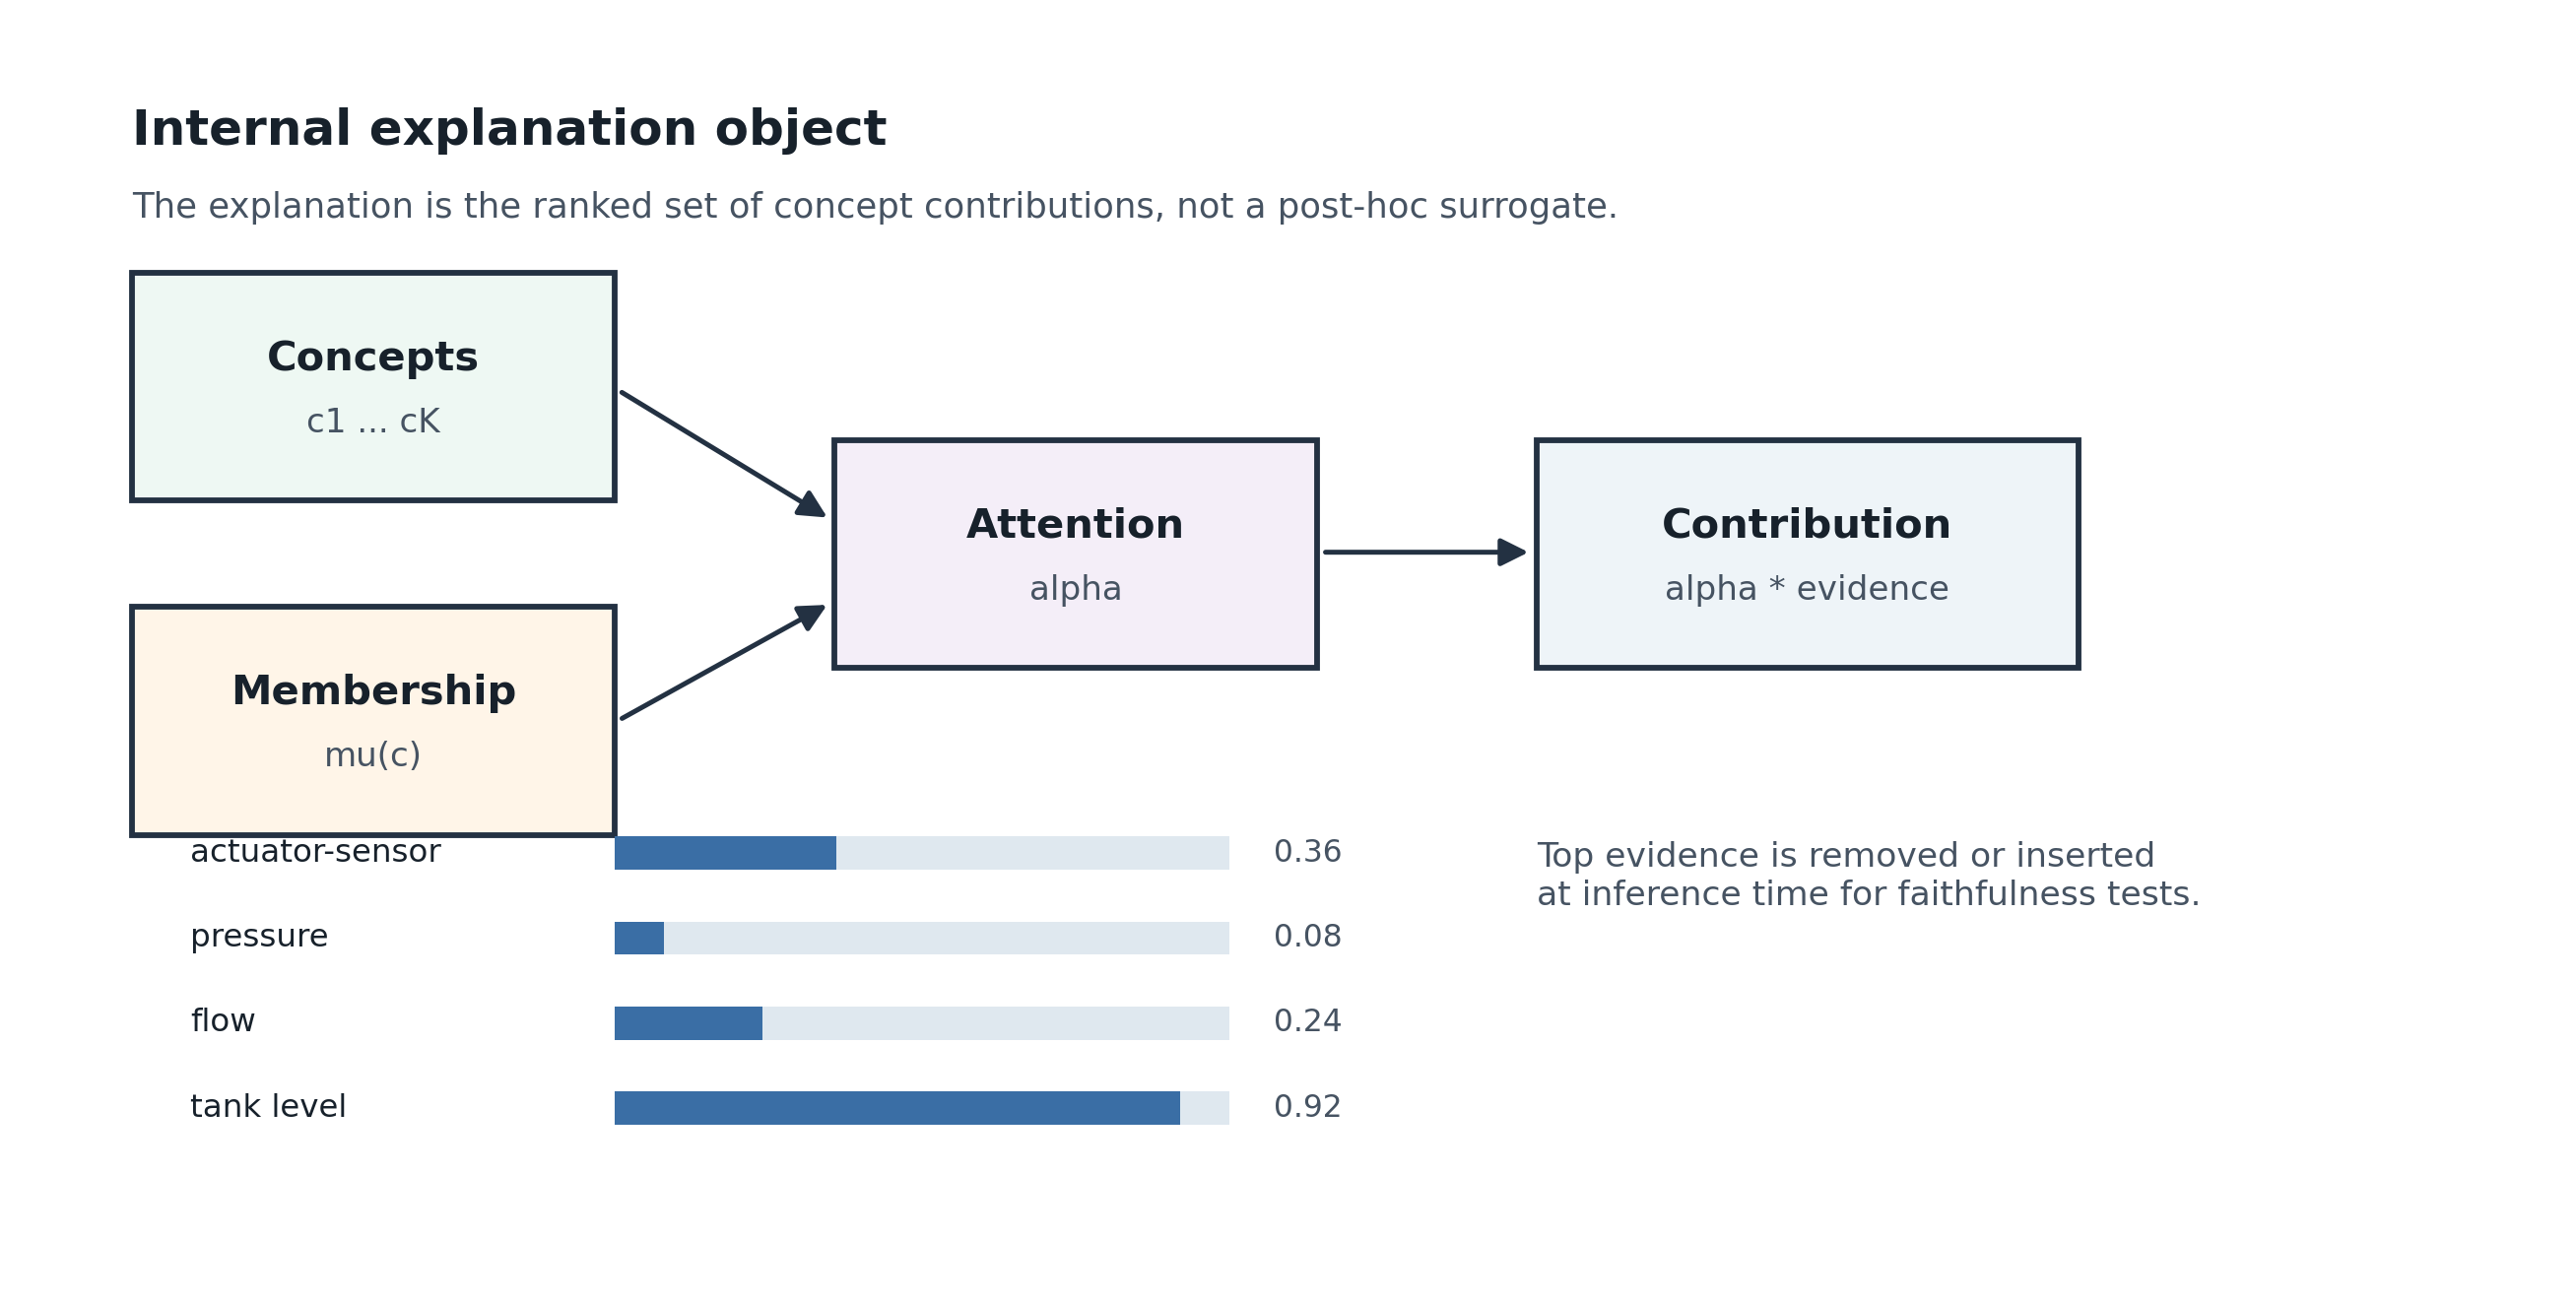
\includegraphics[width=0.86\textwidth]{figures/interpretability_scheme.png}
    \caption{Concept-level explanation and faithfulness test principle.}
    \label{fig:interpretability_scheme}
\end{figure}

From this standpoint, the framework combines the adaptive capacity of deep representation learning with the semantic discipline of concept-oriented reasoning. The encoder provides the ability to learn from complex temporal data, the concept layer imposes an interpretable intermediate organization, and the FAN block transforms concept activations into weighted fuzzy evidence suitable for safety-critical decision support.

\subsection{Concept Definition and Grounding}

A key requirement of the proposed framework is that concepts should not be arbitrary latent dimensions with post hoc names. Each concept is defined before model training as a domain-motivated semantic state derived from observable variables. The concept layer is therefore supervised by soft concept targets constructed from structured transformations of the input signals.

Let $\mathcal{K}=\{1,\dots,K\}$ denote the set of concepts. For each concept $k$, a semantic descriptor is specified in the form
\begin{equation}
\Gamma_k = \left( V_k, \rho_k, \eta_k \right),
\end{equation}
where $V_k$ is the subset of observed variables associated with the concept, $\rho_k(\cdot)$ is a domain-motivated transformation of these variables, and $\eta_k$ denotes the smoothing parameter used to construct the concept target. The corresponding soft concept target is defined as
\begin{equation}
\tilde{c}_k =
\sigma\!\left(
\frac{\rho_k(x_{V_k})-\gamma_k}{\eta_k}
\right),
\end{equation}
where $\sigma(\cdot)$ is the sigmoid function, $\gamma_k$ is a concept-specific reference threshold, and $\eta_k>0$ controls the smoothness of the transition between low and high concept activation.

This formulation allows concept targets to be constructed without requiring hard binary rule activation. Instead, each target concept is represented as a graded value in $[0,1]$, reflecting the degree to which the current observation corresponds to a semantically meaningful system state. For the cyber-physical process monitoring task, the concept set includes tank-level deviation, flow instability, pressure instability, and actuator--sensor inconsistency. For the degradation-aware equipment monitoring task, the concept set includes operational stress, efficiency loss, thermal degradation, and pressure-related instability.

The current prototype uses heuristic domain-motivated transformations of observed variables to construct $\tilde{c}$. These transformations are not claimed to constitute a complete expert knowledge base. However, they make the concept supervision mechanism explicit, reproducible, and tied to observable system variables. This is essential for distinguishing the proposed concept layer from a free latent bottleneck and for supporting semantic inspection of the resulting explanations.

The concept grounding principles for the two datasets are summarized in Tables~\ref{tab:concept_grounding_swat} and~\ref{tab:concept_grounding_fd001}. These tables specify the semantic role of each concept and its relation to observable variables.

\begin{table}[tbp]
\caption{Definition and grounding of SWaT concepts.}
\label{tab:concept_grounding_swat}
\centering
\scriptsize
\setlength{\tabcolsep}{4pt}
\renewcommand{\arraystretch}{1.15}
\begin{tabularx}{\textwidth}{p{0.30\textwidth} X}
\toprule
Concept & Grounding and semantic interpretation \\
\midrule
Tank-level deviation &
Derived from level-related sensors; represents abnormal deviation of tank level from the expected operating range. \\

Flow instability &
Derived from flow-related sensors; represents irregular or abrupt changes in process flow dynamics. \\

Pressure instability &
Derived from pressure-related sensors; represents abnormal pressure behavior associated with process instability. \\

Actuator--sensor inconsistency &
Derived from actuator states and sensor readings; represents mismatch between commanded actuator state and observed physical response. \\
\bottomrule
\end{tabularx}
\end{table}

\begin{table}[tbp]
\caption{Definition and grounding of NASA FD001 concepts.}
\label{tab:concept_grounding_fd001}
\centering
\scriptsize
\setlength{\tabcolsep}{4pt}
\renewcommand{\arraystretch}{1.15}
\begin{tabularx}{\textwidth}{p{0.30\textwidth} X}
\toprule
Concept & Grounding and semantic interpretation \\
\midrule
Operational stress &
Derived from operational settings and sensor variables; represents an operating regime associated with increased mechanical or thermodynamic load. \\

Efficiency loss &
Derived from temperature, pressure, and rotational variables; represents degradation patterns associated with reduced engine efficiency. \\

Thermal degradation &
Derived from temperature-related variables; represents thermal behavior associated with progressive equipment degradation. \\

Pressure instability &
Derived from pressure-related variables; represents pressure-related deviation associated with abnormal operating or degradation behavior. \\
\bottomrule
\end{tabularx}
\end{table}

\subsection{Mathematical Formulation}

Let $\mathcal{X}$ denote the observation space and let $x \in \mathcal{X}$ denote an input sample describing the current state of a monitored system. The decision support task is defined as the construction of a mapping
\begin{equation}
\mathcal{F} : \mathcal{X} \rightarrow \mathcal{Y},
\end{equation}
where $\mathcal{Y}$ denotes the target decision space. Depending on the application, $\mathcal{Y}$ may correspond to anomaly detection, risk estimation, fault-related classification, or another safety-relevant predictive output. In the proposed formulation, the mapping $\mathcal{F}$ is required to satisfy two conditions: predictive adequacy and semantic traceability of decision formation.

The first stage of the model is a trainable encoder
\begin{equation}
f_{\theta} : \mathcal{X} \rightarrow \mathcal{Z},
\end{equation}
which maps the input observation into a latent representation
\begin{equation}
z = f_{\theta}(x), \qquad z \in \mathcal{Z},
\end{equation}
where $\mathcal{Z}$ is the latent representation space and $\theta$ are encoder parameters.

An intermediate concept space $\mathcal{C}$ is introduced to represent semantically meaningful system states. Let
\begin{equation}
g_{\phi} : \mathcal{Z} \rightarrow \mathcal{C}
\end{equation}
denote the latent-to-concept mapping, parameterized by $\phi$. The concept representation is defined as
\begin{equation}
c = g_{\phi}(z), \qquad c = (c_{1}, \dots, c_{K})^{\top} \in [0,1]^K.
\end{equation}
Here, $c_k$ represents the predicted activation of the $k$-th concept. In contrast to an arbitrary bottleneck layer, $\mathcal{C}$ is constrained by concept targets $\tilde{c}$ derived from observable variables and domain-motivated transformations. This follows the general motivation of concept-based intermediate modeling \cite{koh2020cbm}, but extends it by introducing FAN-based fuzzy concept-level evidence aggregation.

Concept consistency is imposed through the discrepancy between predicted concept activations and grounded concept targets:
\begin{equation}
\mathcal{L}_{\mathrm{concept}} =
d_{\mathrm{c}}\!\left(g_{\phi}(f_{\theta}(x)), \tilde{c}\right),
\end{equation}
where $d_{\mathrm{c}}(\cdot,\cdot)$ is a concept-level discrepancy measure. In the prototype implementation, mean squared error is used for continuous soft concept targets. This term forces the concept layer to preserve correspondence with predefined semantic states rather than drifting toward unconstrained latent factors.

To make concept--latent alignment more explicit, an additional structural alignment term is introduced at the level of pairwise similarities. Let $S_Z$ denote the similarity matrix between latent representations in a mini-batch and let $S_C$ denote the similarity matrix between the corresponding concept representations:
\begin{equation}
(S_Z)_{ij} = \operatorname{sim}(z_i,z_j), \qquad
(S_C)_{ij} = \operatorname{sim}(c_i,c_j).
\end{equation}
The latent--concept structural alignment term is then defined as
\begin{equation}
\mathcal{L}_{\mathrm{align}} =
\left\| S_Z - S_C \right\|_{F}^{2},
\end{equation}
where $\|\cdot\|_{F}$ is the Frobenius norm. This term does not assume a bijective or geometry-preserving isomorphism between $\mathcal{Z}$ and $\mathcal{C}$. Rather, it encourages local relational consistency between the latent organization learned by the encoder and the concept-level organization used for decision formation.

\subsection{Fuzzy Concept Attention Mechanism}

Decision formation is performed from the concept representation rather than directly from the latent representation. For this purpose, the proposed model uses a Fuzzy Attention Network as a concept-level evidence aggregation mechanism. The fuzzy character of the mechanism is expressed through graded concept memberships and context-dependent weighting of concept evidence.

For each concept $k$, the predicted concept activation $c_k$ is interpreted as the input to a membership function:
\begin{equation}
\mu_k = m_k(c_k), \qquad \mu_k \in [0,1],
\end{equation}
where $m_k(\cdot)$ denotes the membership function associated with the $k$-th concept. In the implementation, several differentiable membership families are supported. The Gaussian and bell-shaped variants are defined as
\begin{equation}
\mu^{\mathrm{G}}_k =
\exp\!\left(
-\frac{(c_k-\beta_k)^2}{2\delta_k^2}
\right),
\qquad
\mu^{\mathrm{B}}_k =
\frac{1}{1+\left((c_k-\beta_k)/\delta_k\right)^2},
\end{equation}
where $\beta_k$ and $\delta_k$ are learnable center and width parameters. A sigmoid membership $\mu^{\mathrm{S}}_k=\sigma((c_k-\beta_k)/\delta_k)$ is also supported. The main reported variant uses a learnable mixed membership
\begin{equation}
\mu_k =
\omega_{\mathrm{G}}\mu^{\mathrm{G}}_k
+ \omega_{\mathrm{B}}\mu^{\mathrm{B}}_k
+ \omega_{\mathrm{S}}\mu^{\mathrm{S}}_k,
\qquad
\omega=\operatorname{softmax}(u),
\end{equation}
where $u$ is a learnable vector of mixture logits. This formulation preserves differentiability while allowing concept activations to be interpreted as graded degrees of membership in semantically meaningful system states.

The FAN block computes a relevance score for each concept using both its membership value and the context provided by the full concept vector:
\begin{equation}
s_k = r_{\omega}(\mu_k, c),
\end{equation}
where $r_{\omega}(\cdot)$ is a trainable relevance function. In the prototype implementation, $r_{\omega}$ is implemented as a lightweight neural scoring module over the concatenated concept and membership vectors. The resulting fuzzy attention weights are obtained by normalized exponentiation:
\begin{equation}
\alpha_k =
\frac{\exp(s_k/\tau)}
{\sum_{j=1}^{K}\exp(s_j/\tau)},
\end{equation}
where $\tau>0$ is a temperature parameter controlling the sharpness of concept selection. The weighted concept evidence is then defined as
\begin{equation}
h = \alpha \odot \mu,
\end{equation}
where $\mu=(\mu_1,\dots,\mu_K)^{\top}$ and $\odot$ denotes elementwise multiplication. The final decision support output is produced by
\begin{equation}
\hat{y} = q_{\psi}(h),
\end{equation}
where $q_{\psi}$ is the decision function with parameters $\psi$.

Consequently, the overall predictive mapping takes the form
\begin{equation}
\hat{y}
=
q_{\psi}\!\left(
\alpha(g_{\phi}(f_{\theta}(x))) \odot
\mu(g_{\phi}(f_{\theta}(x)))
\right).
\end{equation}

This mechanism differs from conventional attention in two respects. First, attention is not applied to hidden features, temporal positions, or tokens, but to semantically grounded concept memberships. Second, the weighted objects are not arbitrary latent vectors but concept-level evidence units with an explicit interpretation. The mechanism also differs from a standard concept bottleneck model. In a concept bottleneck model, concepts serve as intermediate variables for prediction; in the proposed framework, concepts are additionally transformed into fuzzy memberships and weighted by a FAN block in order to model context-dependent concept relevance.

The interpretable rationale of the decision can therefore be represented by the ordered set
\begin{equation}
\mathcal{E}(x) =
\left\{
(c_k,\mu_k,\alpha_k,\alpha_k\mu_k)
\;\middle|\;
k=1,\dots,K
\right\}.
\end{equation}
In practice, the explanation can be summarized by the top-ranked subset
\begin{equation}
\mathcal{E}_{m}(x)
=
\operatorname{TopM}\left(\alpha \odot \mu\right),
\end{equation}
where $\operatorname{TopM}(\cdot)$ returns the $m$ concepts with the largest weighted contribution to the decision. Under this interpretation, explanation is derived from the internal decision pathway of the model, consistent with the objective of explainable decision support in critical settings \cite{schwalbe2024criticalxai}.

\subsection{Optimization Objective}

The model is trained end-to-end using a joint objective that combines task performance, concept consistency, structural concept--latent alignment, and sparsity of concept-level evidence. The total loss is defined as
\begin{equation}
\mathcal{L}
=
\mathcal{L}_{\mathrm{task}}
+
\lambda_{\mathrm{c}}\mathcal{L}_{\mathrm{concept}}
+
\lambda_{\mathrm{a}}\mathcal{L}_{\mathrm{align}}
+
\lambda_{\mathrm{s}}\mathcal{L}_{\mathrm{sparse}},
\end{equation}
where $\mathcal{L}_{\mathrm{task}}$ is the main task-dependent predictive loss, $\mathcal{L}_{\mathrm{concept}}$ enforces consistency between predicted concepts and grounded concept targets, $\mathcal{L}_{\mathrm{align}}$ encourages structural consistency between latent and concept representations, and $\mathcal{L}_{\mathrm{sparse}}$ controls the concentration of concept-level evidence.

For binary safety-relevant classification tasks, $\mathcal{L}_{\mathrm{task}}$ is implemented as binary cross-entropy:
\begin{equation}
\mathcal{L}_{\mathrm{task}}
=
-\frac{1}{N}\sum_{i=1}^{N}
\left[
y_i\log(\hat{p}_i+\varepsilon)
+
(1-y_i)\log(1-\hat{p}_i+\varepsilon)
\right],
\end{equation}
where $\hat{p}_i$ is the predicted probability, $y_i$ is the target label, and $\varepsilon>0$ is a numerical stabilization constant.

The sparsity term is defined through the entropy of the attention distribution:
\begin{equation}
\mathcal{L}_{\mathrm{sparse}}
=
-\sum_{k=1}^{K}\alpha_k\log(\alpha_k+\varepsilon).
\end{equation}
Minimizing this term encourages more concentrated concept weighting and promotes compact evidence aggregation. This is important for interpretability because explanations based on a small number of dominant concepts are easier to inspect than diffuse explanations distributed across many weakly contributing concepts.

The resulting objective reflects the main methodological assumptions of the framework. The task loss preserves predictive performance, the concept loss grounds the intermediate representation in semantically defined states, the alignment term encourages consistency between latent and concept organizations, and the sparsity term promotes compact concept-level explanations.

\subsection{Prototype Realization and Evaluation Design}

The proposed framework was instantiated as a prototype implementation intended to examine whether the concept-oriented organization described above can be realized in an operational predictive model. The encoder was implemented as a one-dimensional convolutional network operating on multivariate temporal windows. The concept layer was implemented as a learned projection from the latent representation into a fixed-dimensional concept space. The FAN block was implemented as a differentiable concept-level fuzzy attention module producing context-dependent concept weights.

The prototype should be interpreted as a proof-of-concept realization rather than as a complete engineering embodiment. The concept targets are derived from structured transformations of observed variables rather than from a fully externalized expert knowledge base. Nevertheless, the concepts are explicitly defined before training and are tied to observable variables, which makes the concept supervision mechanism reproducible and semantically inspectable.

The empirical evaluation was designed around two complementary safety-relevant scenarios. The first scenario corresponds to anomaly-aware monitoring in a cyber-physical process environment and was examined on the SWaT benchmark \cite{kaggle_swat_dataset}. The second scenario corresponds to degradation-aware risk prediction in equipment health monitoring and was examined on the NASA C-MAPSS FD001 turbofan benchmark \cite{kaggle_nasa_cmaps}. These datasets were selected because they represent two different types of safety-relevant time-series problems: abnormal process behavior and progressive technical degradation.

For each dataset, input observations were transformed into fixed-length temporal windows. Each window was assigned a task label and a vector of soft concept targets. Model development relied on training and validation partitions, model selection was performed using validation F1-score with early stopping, and the final comparison was reported on held-out test data.

The revised evaluation protocol compares the proposed FAN-based concept-oriented model with three baselines. The first is a black-box 1D CNN using the same temporal encoder family but without concept-level organization. The second is a concept bottleneck model (CBM) with the same encoder and concept predictor, followed by a classifier over concepts without FAN-based fuzzy aggregation. The third is a lightweight Transformer encoder that represents an attention-based temporal baseline without explicit concept grounding. This comparison separates the contribution of concept prediction, fuzzy concept aggregation, and generic attention.

A limited component-level ablation study was additionally conducted on SWaT. The evaluated variants include the full FAN-based model, a model without the FAN block, a model without the concept loss, and a model without the entropy-based sparsity term. These variants were selected to test whether concept supervision, FAN-based aggregation, and concentration of concept evidence contribute to the observed predictive behavior.

The principal predictive metrics are accuracy, precision, recall, F1-score, and ROC-AUC. All final comparisons are reported as mean, standard deviation, and 95\% confidence interval over three random seeds. In addition to aggregate predictive performance, representative concept-level explanations were inspected for selected correctly classified and misclassified samples.

Faithfulness is evaluated by concept intervention at inference time. In the removal-based test, the top-ranked concepts are zeroed out and the decrease in predictive quality is measured. In the insertion-based test, only the top-ranked concepts are retained. A faithful concept-level explanation should show a stronger performance drop under removal of dominant concepts and a stronger performance retention under insertion of the same concepts than would be expected from diffuse or irrelevant concept rankings.

\section{Results}

The empirical evaluation indicates that the first prototype realization of the proposed framework is operationally viable in heterogeneous safety-relevant time-series settings. Tables report mean values with 95\% confidence intervals over three random seeds. Across the considered experiments, the proposed architecture maintained competitive predictive quality while introducing a concept-consistent intermediate representation and a concept-level fuzzy attention mechanism into the decision process.

\begin{table}[tbp]
\caption{Multi-seed comparison on SWaT.}
\label{tab:swat_results}
\centering
{\scriptsize\setlength{\tabcolsep}{1.6pt}
\begin{tabular}{lccccc}
\toprule
Model & Accuracy & Precision & Recall & F1-score & ROC-AUC \\
\midrule
CBM & 0.9906 $\pm$ 0.0039 & 0.8387 $\pm$ 0.0689 & 0.9336 $\pm$ 0.0298 & 0.8831 $\pm$ 0.0458 & 0.9927 $\pm$ 0.0004 \\
CNN & 0.9920 $\pm$ 0.0007 & 0.8375 $\pm$ 0.0188 & 0.9785 $\pm$ 0.0091 & 0.9024 $\pm$ 0.0072 & 0.9993 $\pm$ 0.0002 \\
FAN (mixed) & 0.9936 $\pm$ 0.0020 & 0.8751 $\pm$ 0.0485 & 0.9712 $\pm$ 0.0078 & 0.9202 $\pm$ 0.0231 & 0.9993 $\pm$ 0.0001 \\
Transformer & 0.9925 $\pm$ 0.0019 & 0.8500 $\pm$ 0.0418 & 0.9776 $\pm$ 0.0149 & 0.9089 $\pm$ 0.0202 & 0.9990 $\pm$ 0.0002 \\
\bottomrule
\end{tabular}
}
\end{table}

In the anomaly-aware monitoring scenario, the proposed model improved the balance between detection sensitivity and reliability relative to the black-box CNN, CBM, and Transformer baselines, with the clearest gain observed in F1-score. This is particularly relevant in safety-critical settings, where excessive false alarms reduce the practical utility of intelligent decision support.

\begin{table}[tbp]
\caption{Multi-seed comparison on NASA FD001.}
\label{tab:fd001_results}
\centering
{\scriptsize\setlength{\tabcolsep}{1.6pt}
\begin{tabular}{lccccc}
\toprule
Model & Accuracy & Precision & Recall & F1-score & ROC-AUC \\
\midrule
CBM & 0.9814 $\pm$ 0.0020 & 0.7870 $\pm$ 0.0512 & 0.5964 $\pm$ 0.1341 & 0.6720 $\pm$ 0.0675 & 0.9696 $\pm$ 0.0200 \\
CNN & 0.9826 $\pm$ 0.0029 & 0.7822 $\pm$ 0.0470 & 0.6456 $\pm$ 0.0734 & 0.7065 $\pm$ 0.0563 & 0.9837 $\pm$ 0.0007 \\
FAN (mixed) & 0.9831 $\pm$ 0.0016 & 0.7701 $\pm$ 0.0577 & 0.6948 $\pm$ 0.0699 & 0.7279 $\pm$ 0.0272 & 0.9816 $\pm$ 0.0083 \\
Transformer & 0.9838 $\pm$ 0.0044 & 0.7350 $\pm$ 0.0699 & 0.7892 $\pm$ 0.0590 & 0.7606 $\pm$ 0.0594 & 0.9917 $\pm$ 0.0050 \\
\bottomrule
\end{tabular}
}
\end{table}

In the degradation-aware risk prediction scenario, the comparative picture was more balanced. The Transformer achieved the highest F1-score, while the proposed FAN model outperformed the CNN and CBM baselines and remained close to the attention-based baseline. The obtained trade-off suggests that the proposed concept-oriented organization is not restricted to anomaly-oriented monitoring alone and remains feasible under degradation-aware prognostic conditions.

\begin{table}[tbp]
\caption{Limited ablation study on SWaT.}
\label{tab:ablation_swat}
\centering
\begin{tabular}{lccccc}
\toprule
Variant & Accuracy & Precision & Recall & F1-score & ROC-AUC \\
\midrule
Full FAN-based model & 0.9939 & 0.9064 & 0.9356 & 0.9207 & 0.9980 \\
Without FAN & 0.9906 & 0.8734 & 0.8785 & 0.8759 & 0.9840 \\
Without concept loss & 0.9892 & 0.7928 & 0.9693 & 0.8722 & 0.9989 \\
Without entropy term & 0.9928 & 0.8762 & 0.9429 & 0.9083 & 0.9981 \\
\bottomrule
\end{tabular}
\end{table}

A limited ablation study was additionally conducted on SWaT in order to assess the contribution of the main architectural components and regularization terms. The results indicate that the proposed gain is not attributable to a single component alone. Removing FAN reduces the overall balance of concept-level aggregation and leads to a clear decrease in F1-score and ROC-AUC. Removing concept supervision produces a different effect: the model shifts toward a high-recall but lower-precision regime, which substantially reduces F1-score despite preserving high ROC-AUC. Removing the entropy-based concentration term has a milder effect, but still leads to lower precision and F1-score than the full model. Taken together, these observations suggest that the best overall performance is obtained when concept supervision, FAN-based aggregation, and entropy-based concentration are used jointly.

\begin{table}[tbp]
\caption{Removal- and insertion-based concept faithfulness on SWaT.}
\label{tab:faithfulness_swat}
\centering
\begin{tabular}{llccc}
\toprule
Model & Intervention & Top-K & F1 & $\Delta$F1 \\
\midrule
CBM & insert & 1 & 0.8754 $\pm$ 0.0660 & 0.0077 $\pm$ 0.0204 \\
CBM & insert & 2 & 0.8743 $\pm$ 0.0791 & 0.0088 $\pm$ 0.0368 \\
CBM & remove & 1 & 0.9076 $\pm$ 0.0337 & -0.0245 $\pm$ 0.0190 \\
CBM & remove & 2 & 0.6290 $\pm$ 0.6164 & 0.2541 $\pm$ 0.5816 \\
FAN (mixed) & insert & 1 & 0.9355 $\pm$ 0.0087 & -0.0154 $\pm$ 0.0197 \\
FAN (mixed) & insert & 2 & 0.9451 $\pm$ 0.0093 & -0.0250 $\pm$ 0.0276 \\
FAN (mixed) & remove & 1 & 0.1181 $\pm$ 0.1197 & 0.8021 $\pm$ 0.1217 \\
FAN (mixed) & remove & 2 & 0.3304 $\pm$ 0.3239 & 0.5898 $\pm$ 0.3165 \\
\bottomrule
\end{tabular}
\end{table}

\begin{table}[tbp]
\caption{Removal- and insertion-based concept faithfulness on NASA FD001.}
\label{tab:faithfulness_fd001}
\centering
\begin{tabular}{llccc}
\toprule
Model & Intervention & Top-K & F1 & $\Delta$F1 \\
\midrule
CBM & insert & 1 & 0.6730 $\pm$ 0.0693 & -0.0011 $\pm$ 0.0230 \\
CBM & insert & 2 & 0.6722 $\pm$ 0.0698 & -0.0002 $\pm$ 0.0029 \\
CBM & remove & 1 & 0.6714 $\pm$ 0.0496 & 0.0006 $\pm$ 0.0204 \\
CBM & remove & 2 & 0.4976 $\pm$ 0.3328 & 0.1744 $\pm$ 0.4004 \\
FAN (mixed) & insert & 1 & 0.7278 $\pm$ 0.0263 & 0.0000 $\pm$ 0.0101 \\
FAN (mixed) & insert & 2 & 0.6836 $\pm$ 0.0393 & 0.0442 $\pm$ 0.0254 \\
FAN (mixed) & remove & 1 & 0.0507 $\pm$ 0.0096 & 0.6772 $\pm$ 0.0345 \\
FAN (mixed) & remove & 2 & 0.0835 $\pm$ 0.0240 & 0.6444 $\pm$ 0.0429 \\
\bottomrule
\end{tabular}
\end{table}

The faithfulness tests provide quantitative support for the role of concept-level evidence. On SWaT, removing the top-ranked FAN concepts causes a large F1-score drop, while retaining only the dominant concept preserves most of the decision signal. A similar pattern is observed on FD001, where top-concept removal substantially degrades the FAN model. This behavior is weaker for CBM, indicating that FAN produces a more concentrated and intervention-sensitive concept ranking.

\begin{table}[tbp]
\caption{Sensitivity of the proposed FAN to concept membership functions.}
\label{tab:membership_sensitivity}
\centering
\begin{tabular}{lcccc}
\toprule
Membership & SWaT F1 & SWaT ROC-AUC & FD001 F1 & FD001 ROC-AUC \\
\midrule
Gaussian & 0.9095 $\pm$ 0.0209 & 0.9990 $\pm$ 0.0006 & 0.7152 $\pm$ 0.0240 & 0.9823 $\pm$ 0.0010 \\
Bell & 0.9283 $\pm$ 0.0187 & 0.9992 $\pm$ 0.0004 & 0.7138 $\pm$ 0.0571 & 0.9697 $\pm$ 0.0184 \\
Sigmoid & 0.9110 $\pm$ 0.0354 & 0.9986 $\pm$ 0.0005 & 0.7260 $\pm$ 0.0173 & 0.9663 $\pm$ 0.0146 \\
Mixed & 0.9202 $\pm$ 0.0231 & 0.9993 $\pm$ 0.0001 & 0.7279 $\pm$ 0.0272 & 0.9816 $\pm$ 0.0083 \\
\bottomrule
\end{tabular}
\end{table}

The membership-function sensitivity analysis indicates that the proposed concept-level aggregation is not tied to a single handcrafted membership shape. Bell-shaped and mixed memberships provide the strongest SWaT results, while mixed and sigmoid memberships are strongest on FD001. For this reason, the main comparison reports the mixed FAN variant, which provides the most balanced behavior across the two scenarios.

\begin{table}[tbp]
\caption{Representative concept-level explanations for selected SWaT test samples.}
\label{tab:qualitative_swat}
\centering
\scriptsize
\begin{tabularx}{\textwidth}{cllX}
\toprule
Sample & Case & Pred. prob. & Dominant evidence \\
\midrule
0   & Normal & 0.0028 &
actuator--sensor inconsistency (0.4236) $>$ tank-level deviation (0.0016) $>$ pressure instability (0.0000) \\
41  & Attack & 0.9984 &
tank-level deviation (0.9586) $>$ flow instability (0.0001) $>$ pressure instability (0.0000) \\
109 & Attack, pred. Normal & 0.3596 &
tank-level deviation (0.1028) $>$ flow instability (0.0003) $>$ actuator--sensor inconsistency (0.0001) \\
\bottomrule
\end{tabularx}
\end{table}

\begin{table}[tbp]
\caption{Representative concept-level explanations for selected NASA FD001 test samples.}
\label{tab:qualitative_fd001}
\centering
\scriptsize
\begin{tabularx}{\textwidth}{cllX}
\toprule
Sample & Case & Pred. prob. & Dominant evidence \\
\midrule
0    & Low-risk & 0.0238 &
operational stress (0.8661) $>$ efficiency loss (0.0054) $>$ thermal degradation (0.0005) \\
1591 & High-risk, pred. Low-risk & 0.1140 &
operational stress (0.3725) $>$ efficiency loss (0.0287) $>$ pressure instability (0.0009) \\
1593 & High-risk, pred. Low-risk & 0.0870 &
operational stress (0.4371) $>$ efficiency loss (0.0149) $>$ pressure instability (0.0007) \\
\bottomrule
\end{tabularx}
\end{table}

Qualitative inspection of concept-level explanations indicates concentrated concept evidence rather than diffuse latent interactions. As shown in Tables~\ref{tab:qualitative_swat} and~\ref{tab:qualitative_fd001}, normal SWaT windows are predominantly associated with actuator--sensor inconsistency, whereas correctly detected attack windows are dominated by tank-level deviation. In the NASA FD001 setting, both low-risk and misclassified high-risk cases are primarily driven by operational stress, with substantially smaller contributions from the remaining concepts. These examples support the claim that the model operates through sparse and analyzable concept-level aggregation, while also indicating that certain failure cases remain insufficiently separated at the current prototype stage.

\section{Discussion}

The obtained results support the feasibility of organizing safety-critical intelligent decision support through an explicit concept-mediated decision pathway. The main outcome of the study is not limited to the fact that the proposed model achieves competitive predictive performance. More importantly, the experiments indicate that predictive inference can be structured through an intermediate concept representation and a FAN-based concept aggregation mechanism without eliminating the practical usefulness of the model. This is central to the proposed approach: the model is not treated as a black-box predictor supplemented by post hoc explanations, but as a decision architecture in which interpretable concept activations participate directly in the formation of the output.

From a methodological perspective, the proposed framework occupies an intermediate position between classical fuzzy expert systems, concept-based neural models, and conventional attention-based architectures. In contrast to classical fuzzy systems, the proposed model does not require a fully hand-crafted rule base and can learn latent temporal representations from data. In contrast to standard deep models, the final decision is not produced directly from distributed hidden features. In contrast to ordinary concept bottleneck models, the concept representation is not only an intermediate prediction layer, but also the object of context-dependent fuzzy evidence weighting. Finally, in contrast to conventional attention mechanisms, the FAN block operates at the level of semantically grounded concept memberships rather than at the level of opaque latent features, tokens, or temporal positions. This distinction is important because it defines the main novelty of the approach: decision formation is formulated as fuzzy aggregation of concept-level evidence.

The empirical results suggest that the effect of the proposed organization depends on the structure of the decision problem. In the SWaT anomaly-aware monitoring scenario, the proposed model achieved the strongest F1-score among the CNN, CBM, and Transformer baselines. This indicates a more reliable alarm behavior, which is especially relevant for safety-critical monitoring because excessive false alarms can reduce operator trust and weaken the practical value of an intelligent decision support system. The results also show that the gain is not explained only by generic attention, since the Transformer baseline remained below the FAN model in F1-score on this task.

In the NASA FD001 degradation-aware risk prediction scenario, the comparative picture was more balanced. The proposed model outperformed the CNN and CBM baselines in F1-score, while the Transformer baseline achieved the highest overall F1-score. This behavior is consistent with the more gradual and structurally ambiguous nature of degradation processes. Unlike abrupt anomaly detection, degradation-aware risk prediction requires the model to distinguish between normal operating variability and early signs of progressive failure. The results therefore suggest that the proposed concept-oriented architecture is applicable beyond abrupt anomaly detection, but also indicate that degradation-specific concept grounding and temporal modeling should be strengthened in future work.

The ablation results further clarify the role of the main architectural components. Removing the FAN block led to a substantial decrease in F1-score and ROC-AUC, which suggests that concept-level fuzzy aggregation contributes to the predictive behavior of the model rather than only to its explanatory form. Removing concept supervision produced a high-recall but lower-precision regime, indicating that concept consistency helps prevent the model from producing overly broad alarm responses. Removing the entropy-based concentration term had a smaller but still observable effect, reducing the compactness and reliability of the concept-level evidence. These observations support the view that the model benefits from the joint use of concept supervision, FAN-based weighting, and concentration of concept evidence.

The qualitative concept-level explanations provide an initial indication that the model forms decisions through sparse and analyzable evidence. In the SWaT examples, correctly detected attack windows were associated with strong tank-level deviation evidence, whereas a misclassified attack sample showed weaker and less decisive concept evidence. This is important because the explanation mechanism exposes not only successful predictions, but also failure cases in which the model does not activate sufficiently discriminative concepts. In the FD001 examples, operational stress dominated both low-risk and misclassified high-risk cases. This suggests that the current concept set captures relevant operating conditions but may not yet provide sufficient separation between normal operational stress and degradation-specific risk. Thus, the explanations are useful not only for interpreting decisions, but also for diagnosing weaknesses of the current concept design.

At the same time, the present results should be interpreted as evidence of feasibility rather than as final validation of the proposed framework. The first limitation concerns concept grounding. In the current prototype, concept targets are derived from heuristic transformations of observed variables. Although these transformations are explicit and reproducible, they do not yet constitute a fully externalized expert knowledge base. Stronger concept grounding would require expert-defined or hybrid expert--data concept systems, validation of concept semantics, and possibly domain expert assessment of explanation plausibility.

The second limitation concerns the current operational meaning of concept--latent alignment. The proposed formulation constrains latent representations through concept consistency and, in the extended formulation, through structural consistency between latent and concept neighborhoods. However, this does not yet amount to a complete theory of alignment between latent and conceptual spaces. Future work should provide a more rigorous treatment of the relation between latent geometry, concept semantics, and decision-relevant evidence aggregation.

The third limitation concerns the experimental protocol. The current evaluation now includes multi-seed statistics and comparison with CNN, CBM, and Transformer baselines, but a stronger journal-level validation still requires broader comparison with recurrent models, temporal convolutional models, and non-fuzzy concept attention models. A full ablation study should isolate the effects of the concept layer, fuzzy membership functions, FAN weighting, concept supervision, sparsity regularization, structural alignment, and calibration regularization.

The fourth limitation concerns the evaluation of interpretability. The current evaluation includes removal- and insertion-based faithfulness tests, but these tests only cover a first intervention protocol. Future validation should include explanation stability under perturbations, sparsity metrics, calibration of concept activations, and expert-oriented validation. Such evaluation is necessary to demonstrate that the dominant concepts are not merely plausible labels, but are genuinely relevant to the model's decision process under operational variation.

The fifth limitation concerns safety relevance. Although the selected datasets represent safety-relevant monitoring and degradation scenarios, standard classification metrics alone do not fully establish safety-critical suitability. A stronger evaluation should include calibration analysis, robustness under sensor noise and missing data, temporal generalization tests, out-of-distribution evaluation, and cost-sensitive failure analysis. In particular, false negatives and false positives should be analyzed under different operational cost assumptions, since their consequences are not equivalent in safety-critical decision support.

Overall, the study supports the view that interpretable intelligent decision support should be approached as a problem of internal model organization rather than as a post hoc explanation problem alone. The proposed framework provides a prototype-level basis for such an organization by connecting latent representation learning, grounded concept activations, and FAN-based fuzzy evidence aggregation. The current results indicate that this organization can be implemented without sacrificing practical predictive performance, while also producing decision traces that can be inspected at the concept level. Further development should focus on stronger concept grounding, broader empirical validation, quantitative interpretability tests, and safety-oriented evaluation protocols before the framework can be considered ready for deployment-oriented safety-critical applications.

\section{Conclusion}

This study proposed a concept-oriented framework for safety-critical intelligent decision support in which prediction is organized through an explicit sequence of latent representation learning, concept-level representation, and FAN-based fuzzy aggregation of concept evidence. The main methodological contribution is the reformulation of decision formation as a concept-mediated process: the final output is not produced directly from hidden features, but from semantically interpretable concept activations weighted by a Fuzzy Attention Network. In this formulation, interpretability is not treated as an external post hoc procedure, but as a structural property of the predictive architecture.

The proposed framework differs from conventional black-box neural models by introducing an intermediate concept space, from standard concept bottleneck formulations by adding context-dependent fuzzy concept aggregation, and from ordinary attention mechanisms by applying attention to concept-level evidence rather than to opaque latent features. This organization makes it possible to analyze a decision in terms of activated concepts, fuzzy membership-like evidence, and their weighted contribution to the final prediction.

The empirical results demonstrate the feasibility of the proposed organization in two safety-relevant time-series scenarios: anomaly-aware monitoring and degradation-aware risk prediction. In the SWaT setting, the proposed model achieved the strongest F1-score among CNN, CBM, and Transformer baselines, indicating a more reliable alarm behavior. In the NASA FD001 setting, the model outperformed CNN and CBM baselines and remained close to the Transformer baseline, suggesting applicability beyond abrupt anomaly detection. The ablation results further indicate that concept supervision, FAN-based aggregation, and entropy-based concentration jointly contribute to the observed behavior of the model.

At the same time, the current study should be understood as a proof-of-concept rather than as a deployment-ready solution. The concept targets are derived from heuristic transformations of observed variables, which limits semantic fidelity. Future work should incorporate expert-validated concept definitions and extend the evaluation to additional datasets, stronger temporal baselines, calibration analysis, robustness analysis, temporal generalization, and cost-sensitive safety evaluation.

Overall, the study supports the view that interpretable decision support in safety-critical environments should be approached as a problem of internal model organization. The proposed FAN-based concept-oriented framework provides a methodological basis for further development of intelligent decision support systems that combine predictive capacity with semantically structured, concept-grounded, and operationally analyzable decision formation.

\begin{credits}
\subsubsection{\ackname}
The research was carried out within the state assignment of the Ministry of Science and Higher Education of the Russian Federation
(theme No. 124112200072-2).

\subsubsection{\discintname}
The authors have no competing interests to declare that are relevant to the content of this article.
\end{credits}

\begin{thebibliography}{10}
\providecommand{\url}[1]{\texttt{#1}}
\providecommand{\urlprefix}{URL }
\providecommand{\doi}[1]{https://doi.org/#1}

\bibitem{kaggle_nasa_cmaps}
{Behrad3d}: Nasa turbofan jet engine data set (2024), \url{https://www.kaggle.com/datasets/behrad3d/nasa-cmaps}, kaggle dataset, accessed 2026-04-17

\bibitem{chakraborty2025fantf}
Chakraborty, S., Heintz, F.: Enhancing time series forecasting with fuzzy attention-integrated transformers. arXiv preprint arXiv:2504.00070  (2025). \doi{10.48550/arXiv.2504.00070}

\bibitem{koh2020cbm}
Koh, P.W., Nguyen, T., Tang, Y.S., Mussmann, S., Pierson, E., Kim, B., Liang, P.: Concept bottleneck models. In: Proceedings of the 37th International Conference on Machine Learning. Proceedings of Machine Learning Research, vol.~119, pp. 5338--5348. PMLR (2020), \url{https://proceedings.mlr.press/v119/koh20a.html}

\bibitem{onwujekwe2025idss}
Onwujekwe, G., Weistroffer, H.R.: Intelligent decision support systems: An analysis of the literature and a framework for development. Information Systems Frontiers  \textbf{27}(5),  2027--2058 (2025). \doi{10.1007/s10796-024-10571-1}

\bibitem{schwalbe2024criticalxai}
Schwalbe, G., Finzel, B.: Explainable machine learning in critical decision systems: Ensuring safe application and correctness. AI  \textbf{5}(4), ~138 (2024). \doi{10.3390/ai5040138}

\bibitem{trofimov2025fuzzytransformer}
Trofimov, Y.V., Averkin, A.N., Ilin, A.S., Lebedev, A.D., Muravyov, I.P., Shevchenko, A.V.: A fuzzy transformer for multimodal ai: Differential fuzzy attention and adaptive explanations. Soft Measurements and Computing (11), ~3 (2025). \doi{10.36871/2618-9976.2025.11.003}, \url{https://s-lib.com/en/issues/smc_2025_11_a3/}

\bibitem{vaswani2017attention}
Vaswani, A., Shazeer, N., Parmar, N., Uszkoreit, J., Jones, L., Gomez, A.N., Kaiser, {\L}., Polosukhin, I.: Attention is all you need. In: Advances in Neural Information Processing Systems 30. Curran Associates, Inc. (2017), \url{https://proceedings.neurips.cc/paper/2017/hash/3f5ee243547dee91fbd053c1c4a845aa-Abstract.html}

\bibitem{kaggle_swat_dataset}
{Vishal Agrawal}: Swat dataset: Secure water treatment system (2025), \url{https://www.kaggle.com/datasets/vishala28/swat-dataset-secure-water-treatment-system}, kaggle dataset, accessed 2026-04-17

\bibitem{zhang2025hfan}
Zhang, L., Li, Y., Hao, X., Zhang, Q., Yang, A., Guo, J., Zhang, L.: Hypergraph representation learning based on fuzzy attention network. Applied Soft Computing  \textbf{183},  113602 (2025). \doi{10.1016/j.asoc.2025.113602}

\bibitem{zhao2026fanl}
Zhao, Z., Song, D.H., Kim, K.B.: Fuzzy attention convolutional neural networks: A novel approach combining intuitionistic fuzzy sets and deep learning. Computers, Materials \& Continua  \textbf{87}(2), ~32 (2026). \doi{10.32604/cmc.2026.073969}

\end{thebibliography}

\end{document}
